%\documentclass{rspublic_}
\documentclass[a4paper,10pt]{article}
\usepackage[utf8]{inputenc}
\usepackage{url}
\usepackage{float}
\usepackage{times}
\usepackage{multirow}
\usepackage{listings}
\usepackage{paralist}
%\usepackage{epsfig}
\usepackage[figtopcap]{subfigure}
\usepackage[hypertex]{hyperref}



\usepackage{ifpdf}


\newcommand{\I}[1]{\textit{#1}}
\newcommand{\B}[1]{\textbf{#1}}
\newcommand{\BI}[1]{\textbf{\textit{#1}}}
\newcommand{\T}[1]{\texttt{#1}}

\setlength\topmargin{0in}
\setlength\headheight{0in}
\setlength\headsep{0in}
\setlength\textheight{9in}
\setlength\textwidth{6.5in}
\setlength\oddsidemargin{0in}
\setlength\evensidemargin{0in}
\setlength\parindent{0.1in}
\setlength\parskip{0.25em}


%\ifpdf
%  \DeclareGraphicsExtensions{.pdf, .jpg}
% \else
%  \DeclareGraphicsExtensions{.eps, .ps}
%\fi


\usepackage{graphicx}
\usepackage{subfigure}
\usepackage{color}
\newcommand{\note}[1]{ {\textcolor{red} { ***NOTE: #1 }}}
\newif\ifdraft
\drafttrue
\ifdraft
\newcommand{\jhanote}[1]{ {\textcolor{red} { ***shantenu: #1 }}}
\newcommand{\alnote}[1]{ {\textcolor{blue} { ***andre: #1 }}}
\newcommand{\athotanote}[1]{ {\textcolor{green} { ***athota: #1 }}}
\else
\newcommand{\alnote}[1]{}
\newcommand{\jhanote}[1]{}
\newcommand{\athotanote}[1]{}
\fi

\begin{document}
\title{\LARGE Efficient Replica-Exchange Simulations on
  Large-Scale Production Infrastructure}
 
\author{Abhinav Thota$^{1,2}$, Andre Luckow$^{1}$, Shantenu Jha$^{1,2,3}$\\
   \small{\emph{$^{1}$Center for Computation \& Technology, Louisiana State University, USA}}\\
   \small{\emph{$^{2}$Department of Computer Science, Louisiana State University, USA}}\\
   \small{\emph{$^{3}$e-Science Institute, University of Edinburgh, UK}}
   }
 
\maketitle

\section{Introduction}
 
Developing applications that are able to orchestrate heterogeneous
resources across distributed resources is a complex task.  Inevitably,
the design and development of an application is influenced and
constrained by the programming systems and the infrastructure it is
developed against. Breaking this coupling between the development and
the underlying infrastructure, to enable applications to be flexible
(across infrastructure), extensible (to new methods of communication
and coordination) and scalable is an important design objective of
distributed applications -- both logically distributed and physically
distributed.

In this work, we focus on the Replica-Exchange (RE)~\cite{hansmann,Sugita:1999rm} 
methods -- which represent a class of
algorithms that involve a large number of loosely-coupled ensembles.
RE simulations are used to understand physical phenomena -- ranging
from protein folding dynamics to binding affinity calculations. Most RE implementations are either infrastructure specific (Woods et al. 2005)
or, if using multiple distributed resources, they require prior co-scheduling
(Manos et al. 2008). ~\cite{Luckow:2008fp} takes it to the next level and is an example of adaptive RE simulations on production-level grid resources, while ~\cite{parashar_arepex} is an example of \emph{asynchronous} RE simulations, which is based on CometG~\cite{Li:2005:CSC:1090948.1091381}, a decentralized computational infrastructure for Desktop Grid environments.

We develop a flexible, extensible and scalable
implementation of RE that can utilize a range of infrastructure
concurrently (and autonomically/adaptively), that supports different
coordination mechanisms (publish-subscribe, centralised notification),
different replica pairing mechanisms (synchronous versus asynchronous)
and thereby different variants of the RE algorithm. We implement and
demonstrate how a flexible and robust implementation enables the
efficient use of a broad range of infrastructure. We compare and analyze the performance of the different RE models when we scale-up to 256 replicas and scale-out to 4 machines. 
We present results using which the reader can understand which model of RE is most suited for a particular set of resources(distributed, local etc.,)

\alnote{Should we add a section with some scientific background: HIV, Hepatitis...?}
The rest of the paper is organized as follows. Section II presents the different algorithms of RE. Section III  presents the SAGA BigJob architecture which we use to conduct the simulations. In Section IV, we present how each of the RE algorithms are implemented. We also present different implementations of the asynchronous RE algorithm. In Section V, we describe the experiments that we conducted on local and distributed resources. In Section VI, we present the results and analysis. Section VII concludes the paper and discusses future work.

\section{Replica-Exchange Approach}
\label{sec:repex-approach}
The RE algorithm involves the concurrent execution of multiple similar
simulations, the \emph{replicas}.  There is a loose-coupling between
the replicas in form of periodic exchange attempts between paired
replicas. %Previously, we demonstrated the usage of the SAGA Pilot-Job
framework~\cite{saga_bigjob_condor_cloud} -- called the BigJob, to run
RE simulations across multiple, heterogeneous distributed Grid and
Cloud infrastructures~\cite{Luckow:2008fp}.
%\alnote{maybe we should also intro SAGA at some point} \jhanote{Yes} The Simple API for Grid Applications (SAGA)~\cite{saga_gfd90} is an API standardization effort within the Open Grid Forum (OGF)~\cite{ogf_web}, an international standards development body concerned primarily with standards for distributed computing. The various tasks that are carried out using the SAGA APIs include file staging, job spawning and the conduction of the exchange attempts.
%Further, we introduced several adaptivity modes, e.\,g.\ adaptive
%sampling that are able to react to dynamic changes in resource
%availabilities.

%\alnote{Not sure how many technical we need to provide...}  

%Traditionally, depending
%on the number of processes \texttt{N}, the manager creates \texttt{N/2} pairs
%of replicas.  Before launching a job, the manager ensures that all
%required input files are transferred to the respective resource. For
%this purpose, the SAGA File API and the GridFTP adaptor are used. The
%replica jobs are then submitted to the resource using the SAGA CPR
%API and the MIGOL/GRAM middleware.

\subsection{Traditional Replica Exchange}
For the vanilla implementation of RE (Case I), depending
on the number of processes \texttt{N}, the manager creates \texttt{N/2} pairs
of replicas. When the replicas reach a
pre-determined state (e.g. the NAMD job finishes after a fixed number
of steps), a decision as to whether to exchange temperatures between
previously paired replicas is determined using the Metropolis scheme.
The run of an ensemble of replicas in parallel and the subsequent
pairwise exchange attempt are referred to as generation. No two
replicas can belong to different generations. If the exchange attempt
is successful, parameters such as the temperature are swapped. Both
jobs are then relaunched~\cite{Luckow:2008fp}.

The simulation time for an exchange step can be divided into the following components 
- (i) the time to launch the BigJobs, (ii) the queue wait time (first exchange step only) 
($T_{W}$), (iii) the actual runtime of NAMD at each generation ($T_{MD}$), (iv) time spent waiting 
for all replicas to be done ($T_{??}$), (v) the time to make the exchanges at the end of each 
generation, and (vi) the time required to restart the NAMD jobs after each exchange 
step. Steps (iii) to (vi) repeat at after each exchange. We only include steps (i) 
and (ii) for completeness. They only occur at the beginning of the experiment and 
we don't include them in our calculations. We consider the start time as the time 
at which the replicas are launched for the first time. We also think that it is 
safe to say that, irrespective of the implementation details, steps (iii) to 
(vi) are inevitable. \alnote{we should put  behind each step which $T_{x}$ we refer to} 
Putting everything in an equation:

\begin{eqnarray}
T_{TOT} &=& T_{MD} + T_{W} + T_{ME} + T_{R}
\label{eq:equation 1}
\end{eqnarray}

Here, the steps (v) and (vi) occur in a sequential manner.
 
% 1 para limitation on traditional replica exchange
A major limitation of this model is that the replicas are paired in fixed groups. 
Exchanges can only take place between these paired replicas.
This, while limiting the number of replicas which are available for an exchange, also inhibits exchanges between replicas with non-nearest temperatures. This also negates the possibility of crosswalks. A crosswalk is said to occur when a replica originally with a low temperature reaches the upper temperature range and then returns to the lower temperature range. %Moreover, the replicas are attached to their partners, 
%sometimes waiting for them to complete while there are possibly other replicas available which are paired to their partners.
%This also reduces the number of exchanges that can take place within a given time.
Replica pairing works well in an ideal scenario but with heterogeneous systems, 
where the resource availability and performance fluctuates, it is far from ideal. It is 
important to have a scheme that does not depend on a static, well defined \alnote{I think we should explain what well-defined resource model means.}
model of resource availability. This forms the motivation for coming up 
with a formulation that makes it possible to run RE simulations on a range of infrastructures.
 %\jhanote{The point is really the following: Paired-replicas are Ok if
  %it can be guaranteed that equal resources will be available, or the
  %resource availabilty can be predicted in advance. However, in
  %distributed systems, whereby definition, resource availability
  %fluctates it is important to have a scheme/implementation that does
  %not depend on a static, well-defined model of resource availability
  %and execution. This forms the motivation for coming up with a
  %formulation of a well known algorithm that makes it suitable for a
  %range of infrastruture.}
  

  
\subsection{Asynchronous Replica Exchange}
%- Introduce asynchronous Replica Exchange --  1 para on case II and case III (algorithmically)

%To overcome these limitations
We propose an asynchronous RE algorithm similar to Parashar et al.~\cite{parashar_arepex}
where a replica can perform exchanges asynchronously with any other replica in the ensemble. This eliminates the need to pair the replicas and limit exchanges to fixed pairs of replicas. We differ from the model described in Parashar et al. in some important ways. The asynchronous RE model we developed runs on production level grids such as the Teragrid and LONI~\cite{LONI_web}, unlike a specialized infrastructure such as CometG. Also, we run the replicas as MPI jobs. 

Since this is an asynchronous implementation, it is not easy to separate the total simulation time into smaller components. The reason is that many events can occur in parallel at the same time. Distinguishing between serial and parallel events, while (i) the time to launch the BigJobs and (ii) the queue wait time are serial events, (iii) the runtime of NAMD, (iv) the time to make the exchanges at the end of the run of each replica, and (v) the time required to restart the NAMD jobs after each exchange are not. %But we also know that, even in the asynchronous RE model, for particular number of exchanges, each replica needs to restart and run a particular number of times. For example, consider 4 replicas and 16 exchanges. That would mean that, on an average, each replica has to restart 8 times. In this manner, we can calculate the absolute replica runtime. We can also calculate (iv) and (v) 
Here too, we exclude (i) and (ii). Further details depend on the implementation, but we can already see some efficiencies with the asynchronous approach. A tentative equation for total time would be:
\athotanote{how to write the equation with overlapping components?}
\alnote{I would propose to separate the total time-to-solution and the time for a generation. 
In a homogeneous environment we could easily add the times for a generation. In a heterogeneous 
environment we will need something like a speed factor to model this precisely. We should discuss this.}
  \begin{eqnarray}
T_{TOT} &=& [T_{MD} + T_{ME} + T_{R}]
\label{eq:equation 1}
\end{eqnarray}
We implement the asynchronous RE algorithm in two ways: (i) centralized (case II) and (ii) decentralized (case III).

%\athotanote{how do the control flow diagrams
%  look? }
%\alnote{We need to highlight how we particularly differ from Parashar
  %et al: no comet, no MPI jobs, production Grids, understand
  %performance sentence...}
%The asynchronous replica exchange framework builds upon the SAGA BigJob and RE frameworks discussed previously.
%The architecture is shown in Figure 1.
%We present two variants of the Asynchronous RE algorithm. The first is a centralized 
%mechanism where all the replicas are managed by a master. %The master closely monitors the replicas and makes the exchanges when appropriate. 
%The second is a decentralized mechanism where each replica is managed independently, in a decoupled manner.% An agent is launched in place of the replica and will perform the the required actions on behalf of the replica.
%Describe how we implement Case II and Case III (you can use figures)
%using SAGA and the advantages



\section{SAGA BigJob - A Pilot-job Framework}

The Simple API for Grid Applications (SAGA)~\cite{saga_gfd90} is an API that provides the basic functionality required to build distributed applications, tools and frameworks so as to be independent of the details of the underlying infrastructure. SAGA is an API standardization effort within the Open Grid Forum (OGF)~\cite{ogf_web}, an international standards development body concerned primarily with standards for distributed computing. The various tasks that are carried out using the SAGA APIs include file staging, job spawning and the conduction of the exchange attempts.


%%%%% FIGURE %%%%%
 \begin{figure}
\centering
 \subfigure[SAGA BigJob]{
 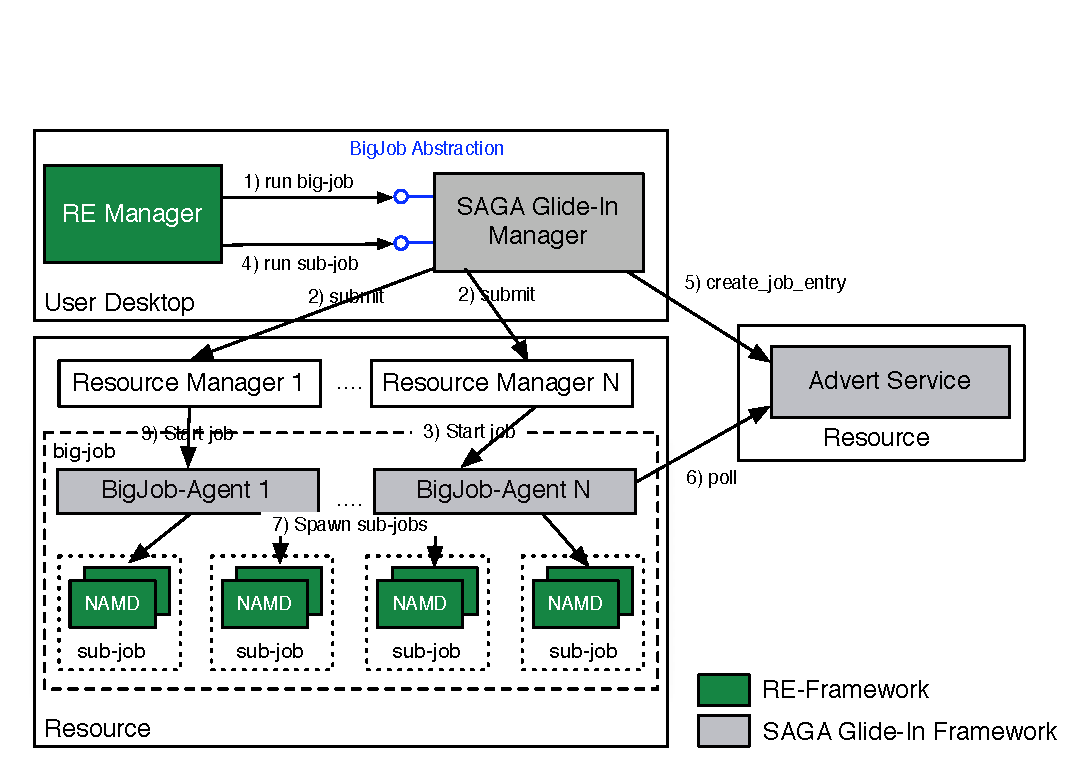
\includegraphics[width=0.45\textwidth]{figures/Bigjob_arch.pdf}
% \caption{\small SAGA/BigJob Architecture}
 \label{fig:bigjob}
 \vspace{-1em}
}%
%
\subfigure[Control Flow: Synchronous Replica Exchange]{
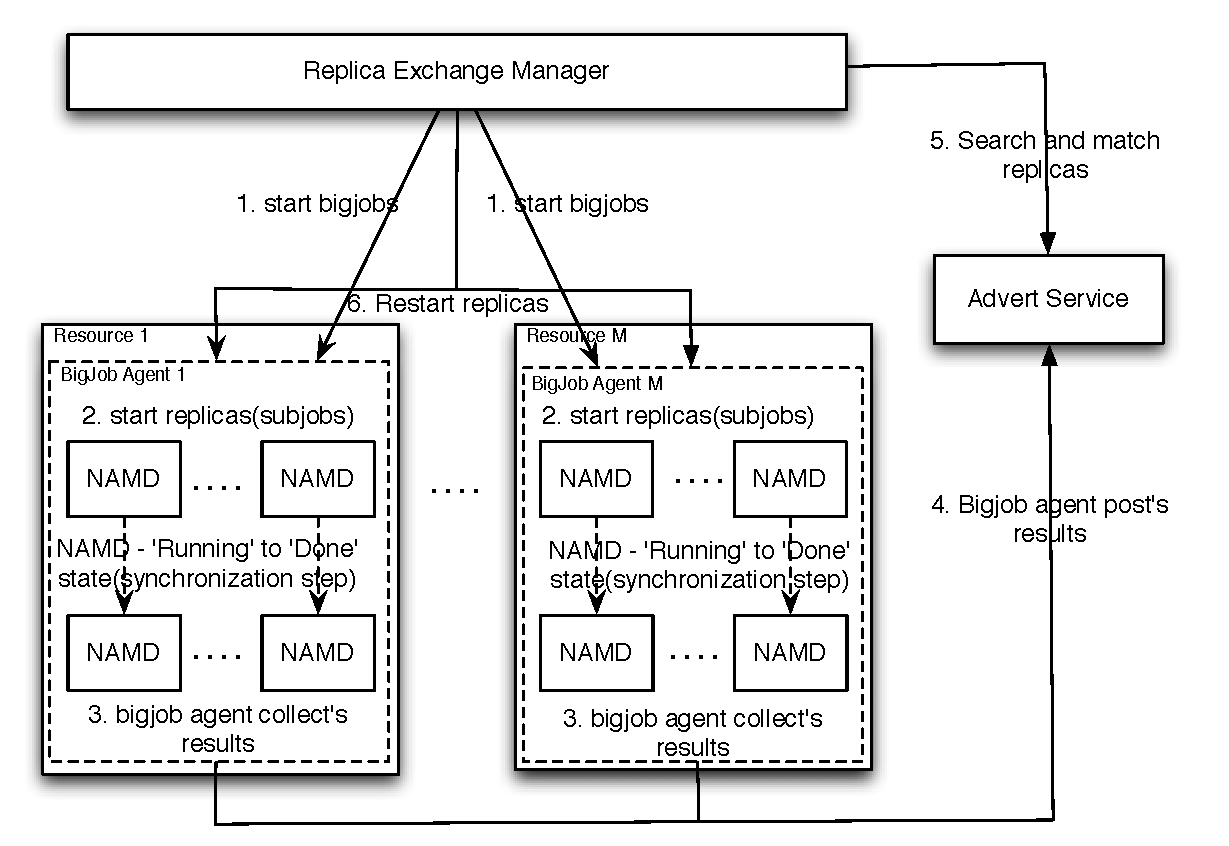
\includegraphics[width=0.45\textwidth]{figures/synchronous.pdf}
\label{fig:sync}
\vspace{-1em}
}
\label{fig:sync}
\caption{\small Caption}
\end{figure}


Previously, we demonstrated the usage of the SAGA Pilot-Job framework~\cite{saga_bigjob_condor_cloud} -- called the BigJob, to run RE simulations across multiple, heterogeneous, distributed grid and cloud infrastructure~\cite{Luckow:2008fp}. Here we are using the SAGA BigJob to efficiently request and manage computational resources. 

\subsection{SAGA BigJob Architecture}

Figure ~\ref{fig:sync}(a), shows the architecture of SAGA BigJob. It consists of three components: (i) the SAGA-BigJob Manager, (ii) the BigJob Agent and (iii) the advert service. The SAGA-BigJob manager submits the BigJobs to the resource manager and the sub-job descriptions to the advert server. Once the BigJobs become active, the BigJob Agent retrieves the job descriptions from the advert server and launches the sub-jobs on each resource. 

\section{Implementation of Synchronous and Asynchronous RE}
We present the implementation details of the Synchronous RE and the two different implementations of the Asynchronous RE algorithm here.

\subsection{Synchronous RE}

In synchronous RE, the master has the overall control of the replicas. 
The first step is to submit a request to the queue for a sufficient 
number of cores for all the replicas (BigJob). A connection to the 
advert server is opened to store job data. The second step is to 
stage the necessary files to the individual working directories. 
In the same step, the job descriptions of each of the replicas are 
posted to the advert server. When the BigJob becomes active, 
a 'bigjob agent' is is launched for each BigJob. The purpose of 
the bigjob agent is to look in the advert server for new replicas 
and to start those replicas. The bigjob agent also monitors the 
replicas under it and posts the status of the replicas to the advert 
server. The master queries the advert server for the latest job 
states and when it find that all the replicas are 'Done', it 
starts making the exchanges. The configuration files are staged 
to the respective working directories. After all the exchanges 
are done in a particular generation, the replica job descriptions 
are posted to the advert server and the bigjob agent restarts the 
replicas. This process is repeated until the required number of 
exchanges are made. 


\subsection{Centralized Asynchronous RE}

%%%%% FIGURE %%%%%
\begin{figure}
\centering
%\subfigure[Control Flow: Centralized Replica Exchange]{
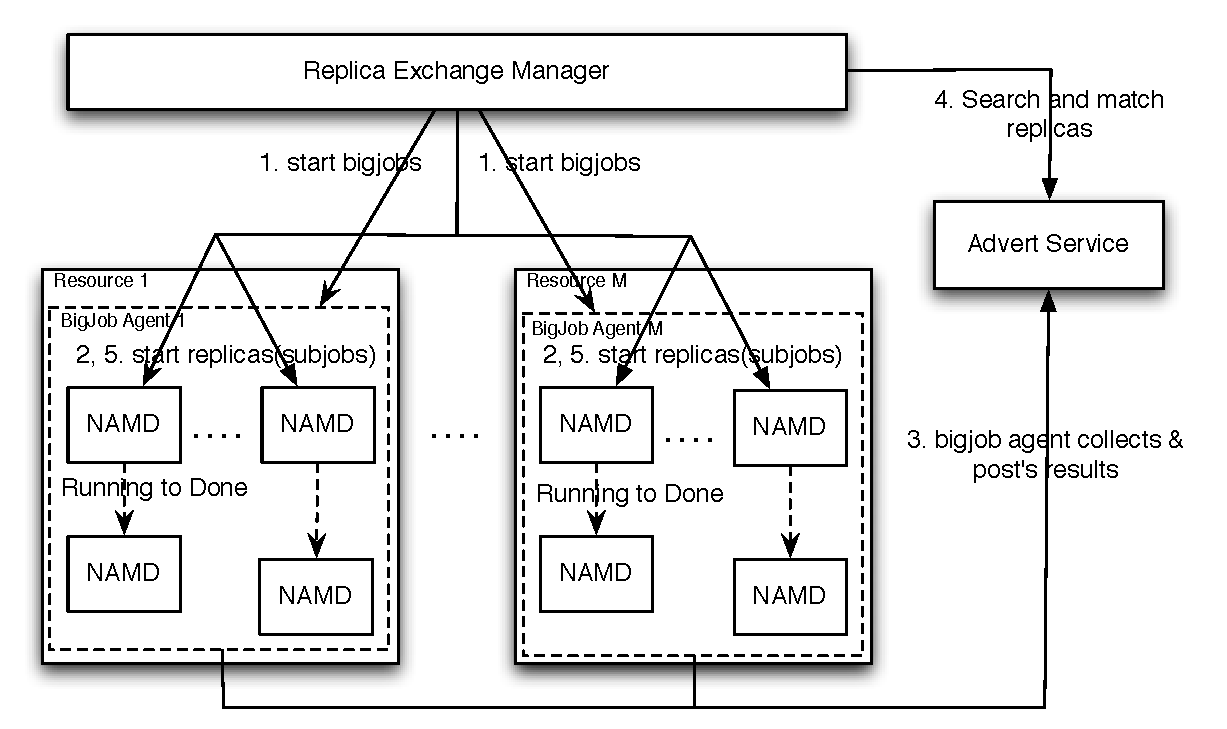
\includegraphics[width=1\textwidth]{figures/centralized.pdf}
%\label{fig:async:b}
\caption{\small In the centralized asynchronous RE (Figure 1(a)) all the replicas are managed by the master, where as in the decentralized asynchronous RE version(Figure 1(b)), for each replica there is a replica agent which individually manages the replica.}
\label{fig:cent}
%\vspace{-1em}
\end{figure}

In the centralized version (Figure~\ref{fig:cent}(a)) of the asynchronous replica exchange (Case II), the master launches and monitors the replicas. The implementation is very similar to that of the synchronous RE, except that the exchanges are done in a asynchronous manner. 

After the initial steps are carried out and the BigJob becomes active, the master searches for replicas in 'Done' state and makes exchanges. \alnote{some more details explaining steps 1-6 would be good.} Again, the configuration files are staged and the job descriptions posted to the advert server for the bigjob agent to restart the replicas.%The decision as to make the exchange or not is made using the Metropolis scheme.  
The process is repeated until the required number of exchanges are made.

\subsection{Decentralized Asynchronous RE}

The decentralized implementation differs from the Cases I and II. We introduce 
a 'replica-agent' for each replica. Each replica-agent manages a single replica. 
Here, the master is limited to the submitting a BigJob request to the queue, 
staging the files. In place of the replica (NAMD executable), the replica-agent 
is launched. The replica-agent is nothing but a wrapper script for the replica. 
At this point, the replica-agent agent starts the replica. The replica-agent 
monitors the replica and posts the state to the advert server. When one of the 
replicas are ready to exchange, they search for another replica which is 
available and negotiate the exchange. There is no need to stage the 
configuration file in this case. \alnote {one could ask why is the 
config file staged in case I and II then?} The data is exchanged over via the 
advert server and the replica agent modifies the configuration file locally.

Although both Case II and Case III implement the asynchronous RE algorithm, they differ in the way they are implemented. The replicas are either managed by a master (Case II) or each replica is managed individually (Case III). We propose Case III so as to not let the master in Case II to become a bottleneck, which can happen very quickly with a large number of replicas.

\begin{figure}
\centering
%\subfigure[Control Flow: Decentralized Replica Exchange]{
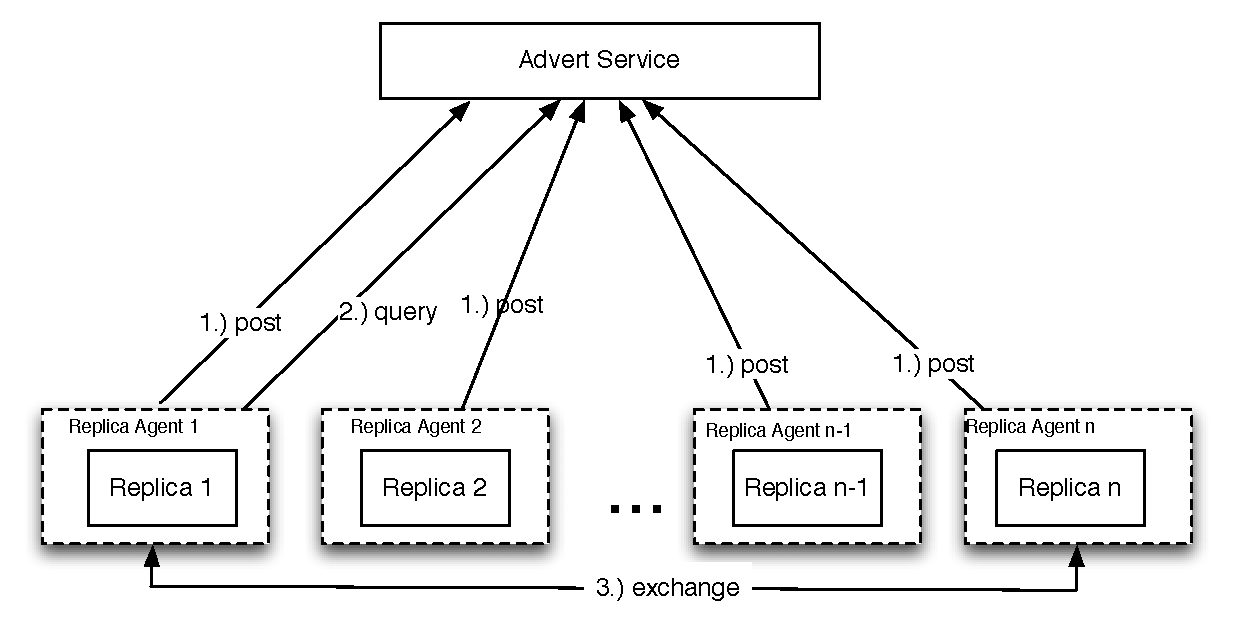
\includegraphics[width=1\textwidth]{figures/asyncre.pdf}
%\label{fig:async:b}
\caption{\small Decentralized control fow.}
\label{fig:decent}
%\vspace{-1em}
\end{figure}

\alnote{we should write Case consistently with small or capital letter}
% We have to bear in mind that while Case II and Case III both implement the same asynchronous RE algorithm, they do it differently.
% At first glance it appears to be a question of philosophy, whether to
% let the replicas be managed by a master or to let each replica be
% managed individually.
%There could be implications effecting the performance of the
%algorithm. Where as in Case II, the master has to manage all the
%replicas and since it can only manage one replica at a time, although negligible, it is a cause for concern with large number of replicas. %The effect could be negligible and might now effect the overall performance.
%But the decentralized version (Case III) has no
%such issues as each replica is managed individually. % \jhanote{The distinction between Case 3 and 2 needs to
%  be made more clear. The following is ``implementation detail''. What
%  is the conceptual difference between Case 3 and Case 2?}

\section{Scale-Up and Scale-Out: Experiments and Results}

%
%%%%% FIGURE %%%%%
\begin{figure}
\centering
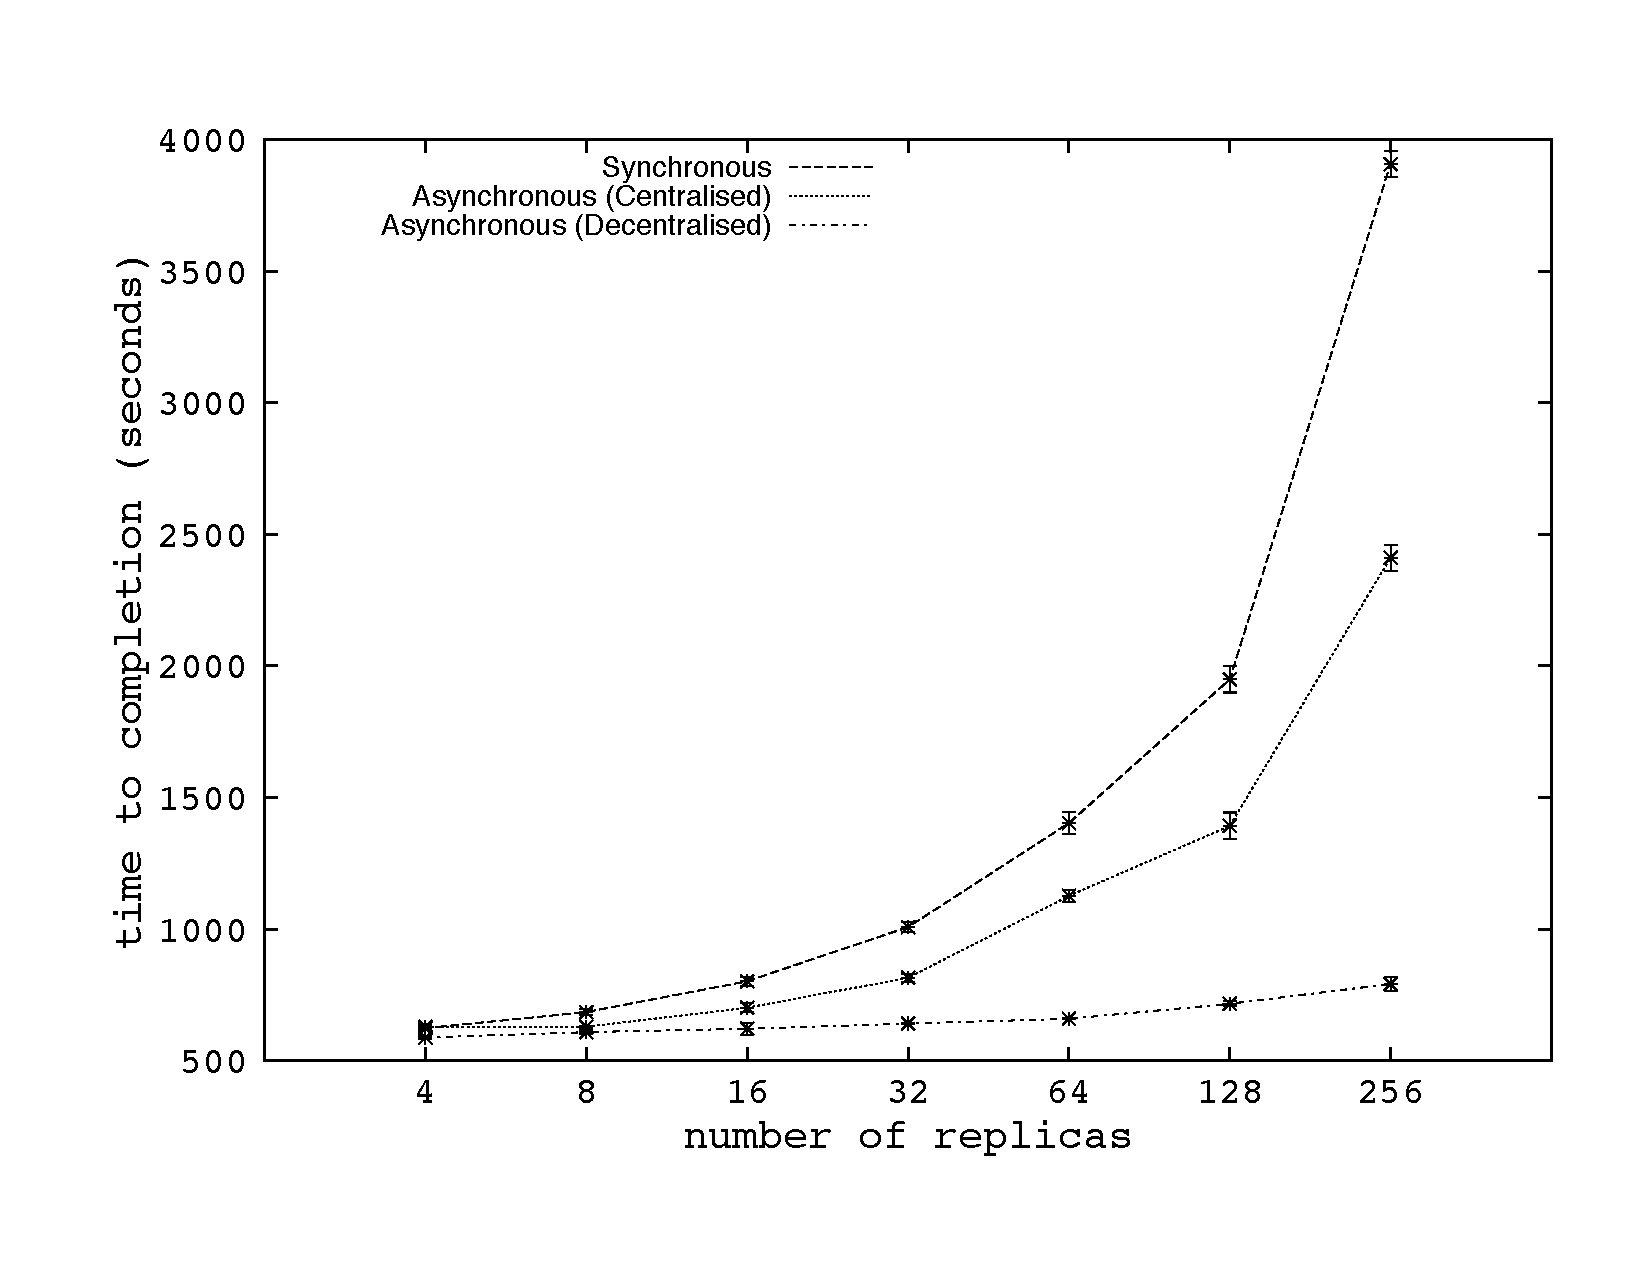
\includegraphics[scale=0.50]{data/scale_up.pdf}
\caption{\small The graph shows the mean run times of synchronous and asynchronous - centralized/decentralized RE simulations on one machine. We repeated the experiments with up to 256 replicas. Up to 128 replicas, the experiments were conducted on QB and 256 replicas experiments were conducted on Ranger.}
\label{fig:graph}
\vspace{-1em}
\end{figure}


%While the traditional RE limits the exchanges to only neighboring temperatures, an asynchronous RE does not. This is not a concern when the number of replicas is small and there is little chance of an exchange between non-adjacent temperatures. However, as the number of replicas increases, the difference between the target temperatures becomes small enough to allow exchanges between non-adjacent temperatures. This also allows for 'crosswalks' to happen. The larger the number of crosswalks, the better is the performance of the simulation.

%To evaluate the performance of the various models of RE we have discussed in the abstract, we conducted several experiments on Teragrid and LONI resources. 
%In the following sentences we will analyze the performance of synchronous RE(Case I) with centralized asynchronous RE(Case II). 

\subsection{Scale-Up}

\subsubsection{Experiments}
We configured the Cases I, II \& III to run parallel NAMD simulations with 4, 8, 16, 32, 64, 128 and 256 replicas sampling a temperature between 300 and 3000 K. \alnote{What resource?} One BigJob is launched with sufficient cores while each replica uses 16 MPI processes and runs 500 time steps between exchange attempts. The metric used is the time to complete 16, 32, 64, 128, 256, 512 and 1024 attempted exchanges, respectively. It should be noted that the ratio between the number of replicas and the number of attempted exchanges is kept constant, for the purpose of comparison between each of these cases.  %Both cases were run over 1, 2 and 4 machines, where the BigJobs are distributed equally across the resources. 
%The initial results suggest that the performance has improved at two levels: (i) the time to completion of Case II is reduced by over 200\% compared to Case I and (ii) there is considerable reduction in the time to completion when running across four machines instead of only 1 machine, by as much as 65\%.

The mean run time is obtained by subtracting the queue wait time of the BigJob from the total time. As the ratio between the number of replicas and number of exchanges is kept constant, ideally, the runtime must remain constant too. In the graph (Figure~\ref{fig:graph}), we see an increase in the time to completion as the number of replicas increases. The increase in the completion time is not uniform across the three cases. We see the most slow down in Case I and the least in Case III.

\subsubsection{Scale up performance: Results and Analysis}

{\it Results:}\\

{\it Analysis: } From the graph (Figure~\ref{fig:graph}), we see that
Case I does not scale very well when we increase the number of
replicas. This is because of an inability to start and end all the
replicas at the same time. With more and more replicas, the
synchronization cost increases.  In Case II, the exchanges happen in
an asynchronous manner, but they are still conducted by the master
alone. As the number of replicas increases, the master quickly becomes
a bottleneck. But in Case III, the exchanges are all carried out in a
decentralized manner. Many exchanges can occur between different pairs
of replicas at the same time. Therefore, we say that the asynchronous
RE algorithm scales better and that the decentralized implementation
is better than the centralized implementation.

%
%%%%% FIGURE %%%%%
\begin{figure}
\centering
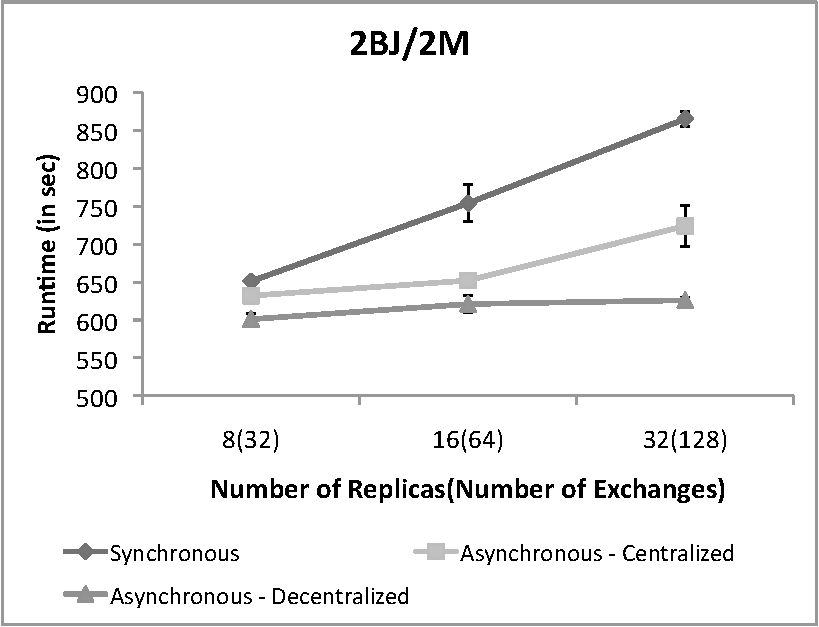
\includegraphics[scale=0.80]{data/2Machines.pdf}
\caption{\small The graph shows the mean run times of synchronous and asynchronous - centralized/decentralized RE simulations across two machines.}
\label{fig:2machines}
\vspace{-1em}
\end{figure}

\begin{figure}
\centering
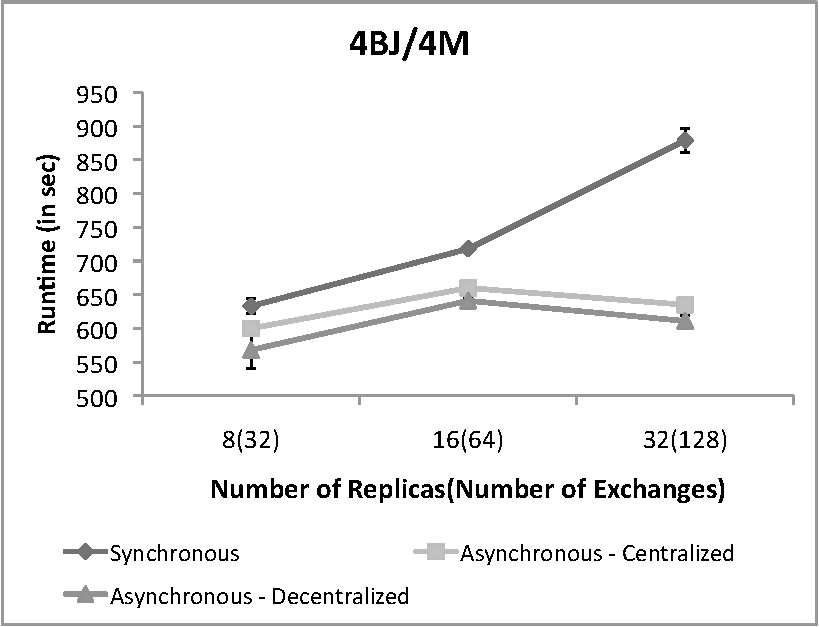
\includegraphics[scale=0.80]{data/4Machines.pdf}
\caption{\small The graph shows the mean run times of synchronous and asynchronous - centralized/decentralized RE simulations across four machines.}
\alnote{maybe it would be good to present both 2m/4m scenario in one graph. Makes the comparison a little easier.}
\label{fig:4machines}
\vspace{-1em}
\end{figure}

\subsection{Scale out performance}
\subsubsection{Experiments}
We chose LONI and Teragrid machines to run Cases I, II \& III. We did experiments distributed across two and four machines. We did these experiments with 8, 16 and 32 replicas distributed equally across two and four machines. 
Figure~\ref{fig:2machines} and Figure~\ref{fig:4machines} show the behavior of Cases I, II and III across one, two and four machines, respectively. On the whole, there is not much difference between the local and distributed runs in any case. The reason being that there is very little interaction between the replicas. A very small configuration file is staged to the remote machines after an exchange, which will not add more than a couple of seconds per exchange. The rest of the co-ordination is done via the advert service, which is usually located on a remote machine in any case. Each query to the advert server is in the order of milli seconds and does not produce a noticeable effect on the performance. 

\subsubsection{Analysis}
In Figure~\ref{fig:2machines}, we see the performance of all three cases when run in a distributed manner across two machines. As the data that is exchanged between replicas is very small, the Cases I, II and III behave in a similar manner to the way they behave on a single machine. \alnote{we should add some numbers and maybe a graph for an example scenario: x: #machines y: time-to-solution} Again, asynchronous RE is better suited for distributed runs and the decentralized implementation scales best. The reason is, since each replica has its own replica agent, there is no need to transfer any files between machines. The required configuration files are created locally by the replica agent.


%In Case I, the pair-wise replica exchange can occur only between replicas of the same generation. Therefore, each exchange step is attempted only after all the replicas have finished running. After the exchange, all the replicas are restarted sequentially. This inserts a delay between the start time of the first replica, the last replica and the replicas in between. %As more resources become available at different times, the replicas already running or done are forced to wait for the newly running replicas to finish before moving on to the next exchange step. %Each exchange step is counted as an exchange.
%In Case II, the pair-wise replica exchange can take place between any two replicas in the ensemble irrespective of generation. As more resources become available, the new replicas join the ensemble immediately and the replicas already running are not restrained from attempting exchanges or restarting. This gives the asynchronous or synchronous RE a slight advantage. But with a large number of replicas we could easily see large difference.
%\athotanote{Further, we show performance gains by running across more than one machine. By running across more than one machine, we demonstrate the ability to divide the jobs into smaller sub-jobs and then distribute them across a number of machines, thereby reducing the risk of long queue wait times on an over-crowded resource. In Figure~\ref{fig:graph}, it can be seen that the asynchronous RE time to completion improves almost by a factor of 3 when moving from one machine to four machines. This was caused due to the fact that when the experiment was done on one machine, by the time the experiment ended, only 64 cores were allocated by the resource manager. But on the other hand, when the experiment was launched across four machines, it received an allocation of 64 cores on each of the four resources. The improvement that is seen in the case of synchronous RE from one to four machines is also due to a similar reason.} %The asynchronous RE appears faster by a couple of minutes due to the fact that when the BigJobs become available randomly, the synchronous RE has to wait for the newly running replicas to finish.

%slightly over 2 machines, but again increases over 4 machines. This is due to the fact that the experiments have been run only a handful of times but, over time, it can be assumed that it will result in reduced queue wait times.

\section{Conclusion}



%\athotanote{is this right? }
% We are also going to have a wider group of replicas to look at for
% each replica as we are not pairing the replicas.

% Also, we have the usual advantages of using a pilot-job,
% such as reduced queue wait times by not having to submit to the queue
% at every step.  We also provide major advantages when compared to
% Parashar et al.

%  to run the asynchronous RE simulations,
% including the ability to run MPI
% jobs.
% ??We need to evaluate the performance of our models and compare with other models for conducting replica exchange simulations.


%%%%% FIGURE %%%%%
%\begin{figure}
%\centering
%\subfigure[Time to complete 64 exchanges on QB with two 64 core BigJobs and on both QB/Louie jointly with a 64 core BigJob on each machine.]{
%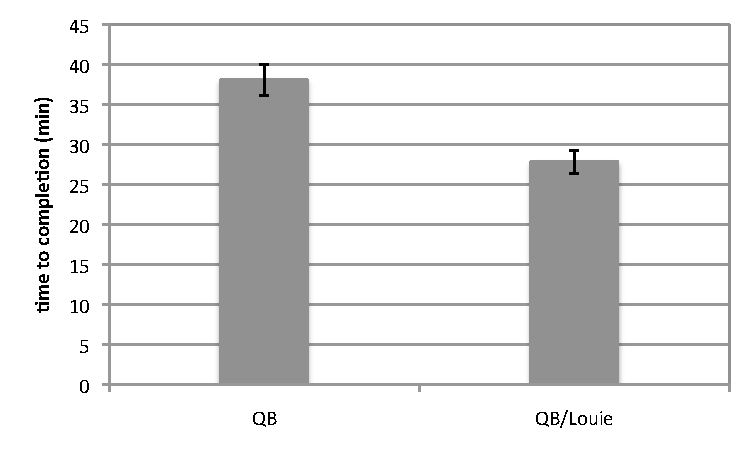
\includegraphics[width=0.40\textwidth]{figures/graph1.pdf}
%\label{fig:subfig3}
%}
%\hspace{0.5cm}
%\subfigure[Time to complete different number of exchanges on QB/Louie with a 64 core BigJob on each machine.]{
%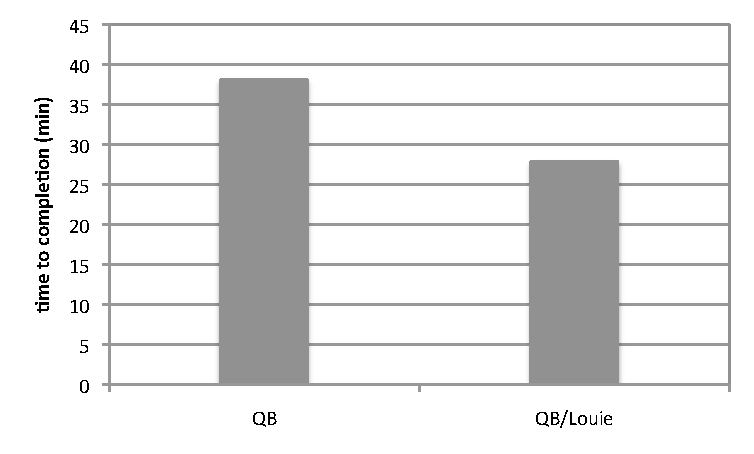
\includegraphics[width=0.40\textwidth]{figures/graph2.pdf}
%\label{fig:subfig4}
%}
%\caption{\small In Figure 2(a), we can see the improvement in performance when run on more than one machine. It is due to the fact that usually the first queued job becomes active before the second on a machine and running jobs on more than one machine solves this problem. In Figure 2(b), we can see consistent performance over prolonged runs, making 32, 64 and 128 exchanges.}
%\label{fig:graphs}
%\vspace{-1em}
%\end{figure}
%%%%% FIGURE %%%%%

An important motivation for this work is to implement a scheme that does not depend on a
static, well defined model of resource availability. %We test and scale
%our implementation on production level grids such as Teragrid and
%LONI~\cite{LONI_web}.
Preliminary results, shown in Figure~\ref{fig:graph}, indicate the most important advantages of asynchronous RE and SAGA/BigJob over traditional RE: (a) allows for exchanges to occur between replicas with non-nearest temperatures, which in turn allows crosswalks to happen (b) a reduced time to completion when running on more than one machine due to improved resource availabilities, (c) the advantage of using a pilot-job mechanism, which eliminates the waiting times at the local resource manager, \alnote{have shown this in prev. papers, but we don't really have data in this one} and (d) the ability to scale out across different production level infrastructure, such as, the Teragrid and LONI.
% It performs well even after doubling and quadrupling the number of
% exchanges required to complete the simulation. The time to
% completion only increases by 35\% after doubling and 117\% after
% quadrupling the number of exchanges.
%\athotanote{should the results
%  be included in the conclusion or in a separate results section? Do
%  you agree with the \# of exchanges scheme to show the data?}
% Unfortunately we have results only for Case II currently, but 

%In summary, we have established the ability to scale-out across different
%infrastructure and compared the performance of the asynchronous
%RE with the synchronous RE at large scales. 
Further, we compare the traditional RE model (Case I) and the centralized (Case II) and decentralized (Case III) models of the asynchronous replica exchange by modeling and repeating the experiments a reasonable number of times, so as to accurately quantify the scientific and performance gains. %We also propose to measure the frequency with which crosswalks occur with increasing number of replicas and measure the advantages due to a decentralized implementation in the full paper.


%With this asynchronous replica exchange mechanism we can improve the
%number of exchanges per unit time, a key parameter in judging the
%performance of a replica-exchange mechanism. \athotanote{is this
 % right? }  We are also going to have a wider group of replicas to
%look at for each replica as we are not pairing the replicas. Also, we
%have the usual advantages of using a pilot-job, such as reduced queue
%wait times by not having to submit to the queue.  Unfortunately we
%dont have results \jhanote{What results can we present -- any? some?},
%so we will say, (i) we establish the ability to scale-out (distributed
%and exa-scale) across different infrastructure (ii) compare the Async
%versus sync formulation at unprecedented scales \jhanote{At least
%  outline what infrastructure we / you are planning to use?} (iii)
%compare different implementations of the Async version
 
 \bibliographystyle{IEEEtran} 
 \bibliography{literature,saga}


\end{document}

